%DIF < \section{Compute-driven, Flight-Efficiency Optimization: A Case Study}
\section{\DIFaddbegin \DIFadd{Compute-driven, Flight-Efficiency Optimization: A }\DIFaddend Case \DIFdelbegin \DIFdel{Studies}\DIFdelend \DIFaddbegin \DIFadd{Study}\DIFaddend }
\label{sec:case-study}

Our closed-loop simulation platform, together with our plug and play benchmarks, enables a holistic inspection of intra-system and system/environment interactions. Studying of the former open doors for hardware/software co-design studies. Such studies starts with the profiling and sensitivity analysis as exemplified in the previous section. The latter enables environment focused considerations and designs such \DIFdelbegin \DIFdel{as reliability studies%DIF < , i.e. the effect of various localization kernels and collision avoidance algorithms on the system. 
}\DIFdelend \DIFaddbegin \DIFadd{reliability studies, i.e. the effect of various localization kernels and collision avoidance algorithms on the system. }\DIFaddend In this section \DIFdelbegin \DIFdel{, we conduct performance, energy and reliability case studies  highlighting the insights architects can take advantage of by using our platform.   
}%DIFDELCMD < \red{\subsection{Sensor-cloud: A Performance Case-Study}
%DIFDELCMD < As opposed to the studies provided in the previous section where our setup emulated a fully-on-edge drone (i.e. a drone which all of its computation is done on the drone itself), our setup can further examine a cloud/edge drone where the computation is distributed across the edge and the cloud. To examine the impact of cloud computing for MAVs, we compare a fully-on-edge drone equipped with a TX2 versus a fully-in-cloud drone with only a minimal computer on board (i.e. a flight controller) but a powerful cloud support (mention the x86 platform we used). This case study targets Mapping as the application of choice. As can be seen in Fig.\ref{fig:edge_cloud}, a drone that can enjoy the cloud's extra compute power sees a 3X speed up in planning time. This improves the average velocity of the drone due to the reduction in hover time and hence reduces the overall mission time almost to half.
%DIFDELCMD < }
%DIFDELCMD < \begin{figure}[t!]
%DIFDELCMD < \centering
%DIFDELCMD < 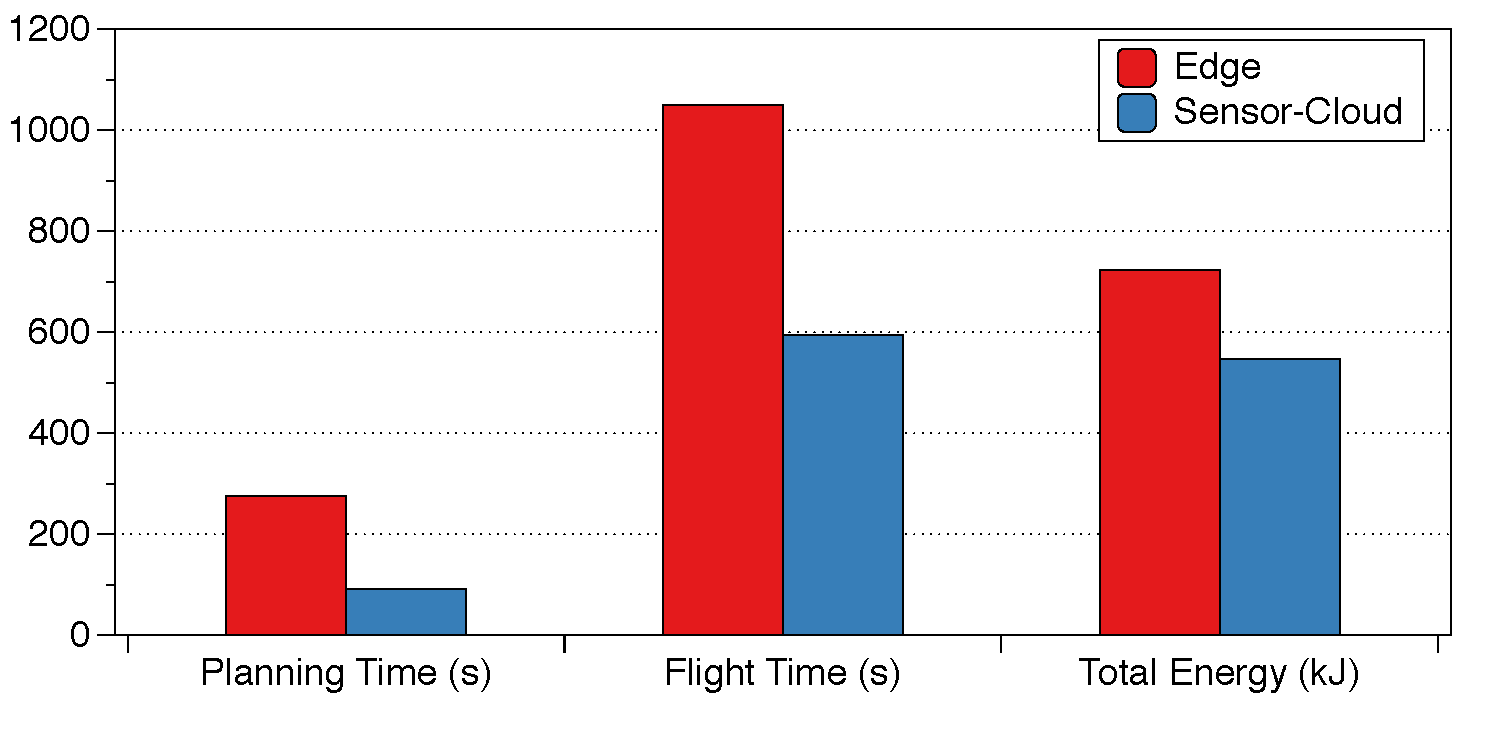
\includegraphics[trim=0 0 0 -25, clip, width=0.9\linewidth]{figs/tx2-desktop}
%DIFDELCMD < %%%
%DIFDELCMD < \caption{%
{%DIFAUXCMD
\DIFdelFL{Comparing a full-on-edge drone vs a full-on-cloud drone.}}
%DIFAUXCMD
%DIFDELCMD < \label{fig:cloud_edge}
%DIFDELCMD < \end{figure}
%DIFDELCMD < %%%
\subsection{\DIFdel{Environment Aware Design: An Energy Case-Study}}  
%DIFAUXCMD
\addtocounter{subsection}{-1}%DIFAUXCMD
\DIFdelend \DIFaddbegin \DIFadd{we consider an example of the latter.   
}

\DIFaddend We conduct a kernel/environment sensitivity analysis using the OctoMap node~\cite{octomap}, which is a major bottleneck in \DIFdelbegin \DIFdel{3 of our end to  applications, namely package package delivery, mapping and search and rescue}\DIFdelend \DIFaddbegin \DIFadd{our benchmark suite}\DIFaddend . OctoMap is used for modeling of various environments without prior assumptions. In order to do so, the map of the environment is maintained in an efficient tree-like data structure while keeping track of the free, occupied and unknown areas. Both planning and collision avoidance kernels utilize this data structure to make safe flights possible by only allowing the drone to navigate through free spaces.  

\DIFdelbegin %DIFDELCMD < \begin{figure}[b]
%DIFDELCMD < \centering
%DIFDELCMD < 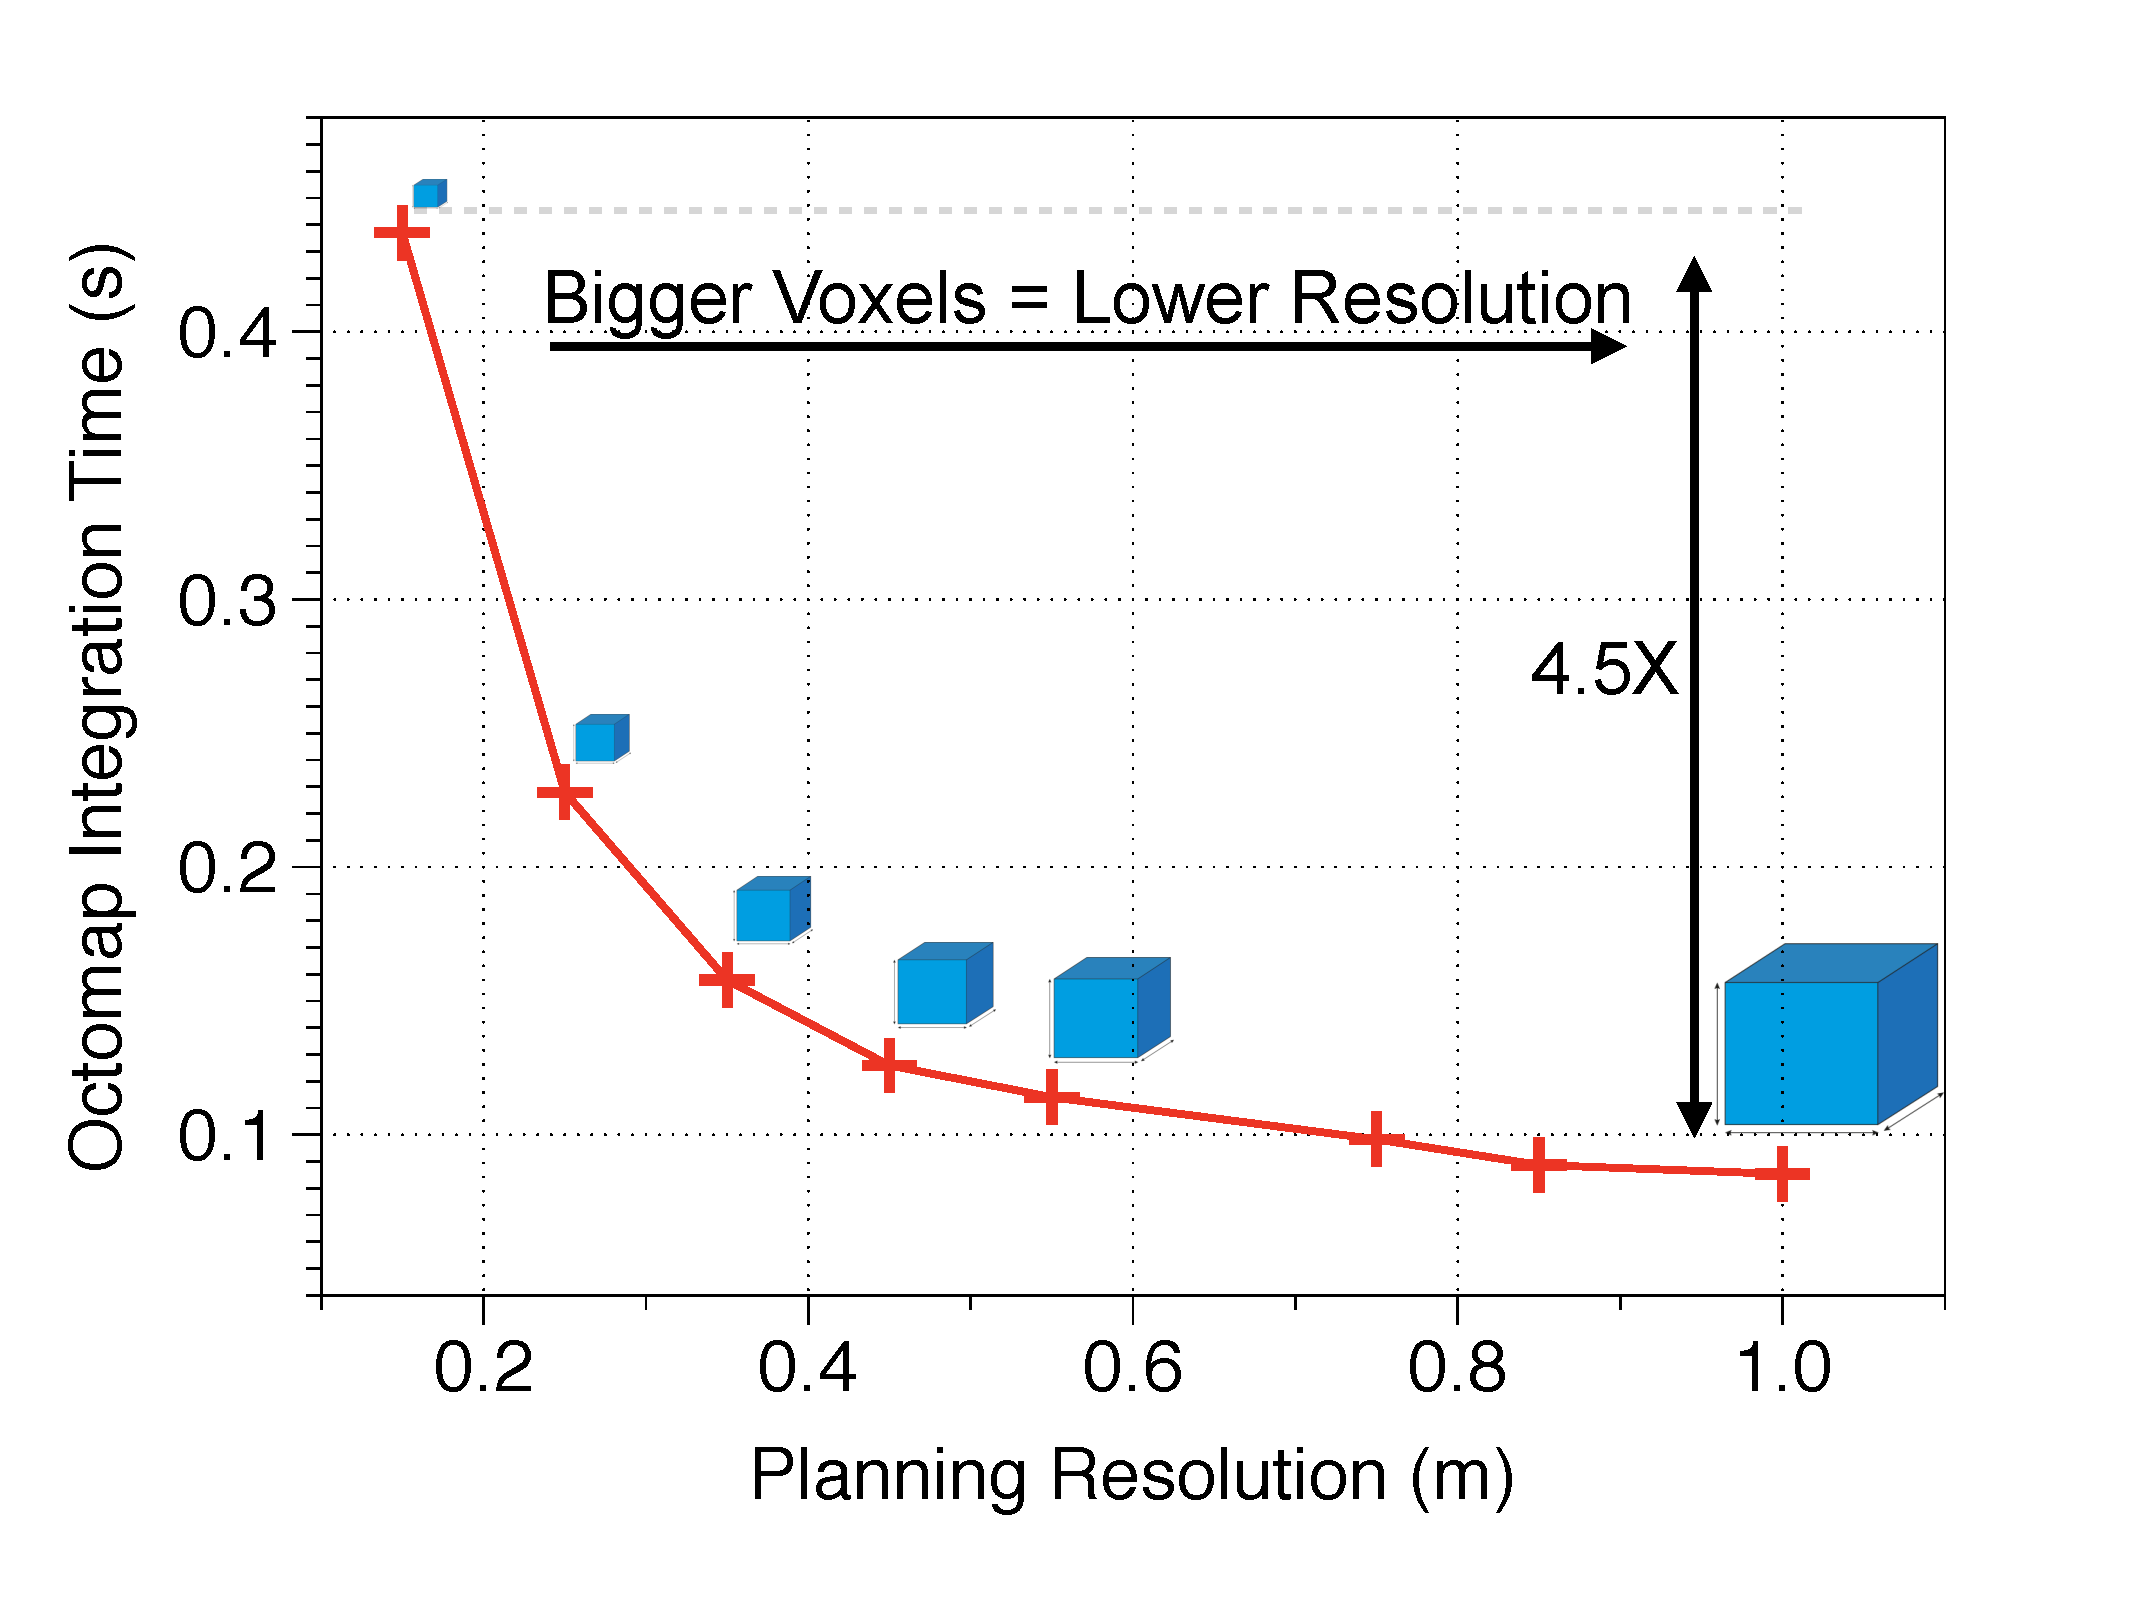
\includegraphics[trim=0 0 0 -25, clip, width=\columnwidth]{figs/octomap_resolution_with_boxes}
%DIFDELCMD < %%%
%DIF < \vspace{-30pt}
%DIFDELCMD < \caption{%
{%DIFAUXCMD
\DIFdelFL{OctoMap accuracy (resolution) versus performance.}}
%DIFAUXCMD
%DIFDELCMD < \label{fig:octrest}
%DIFDELCMD < \end{figure}
%DIFDELCMD < 

%DIFDELCMD < \begin{figure*}[t!]
%DIFDELCMD <     \centering
%DIFDELCMD <     \begin{subfigure}{.23\linewidth}
%DIFDELCMD <         \centering
%DIFDELCMD <         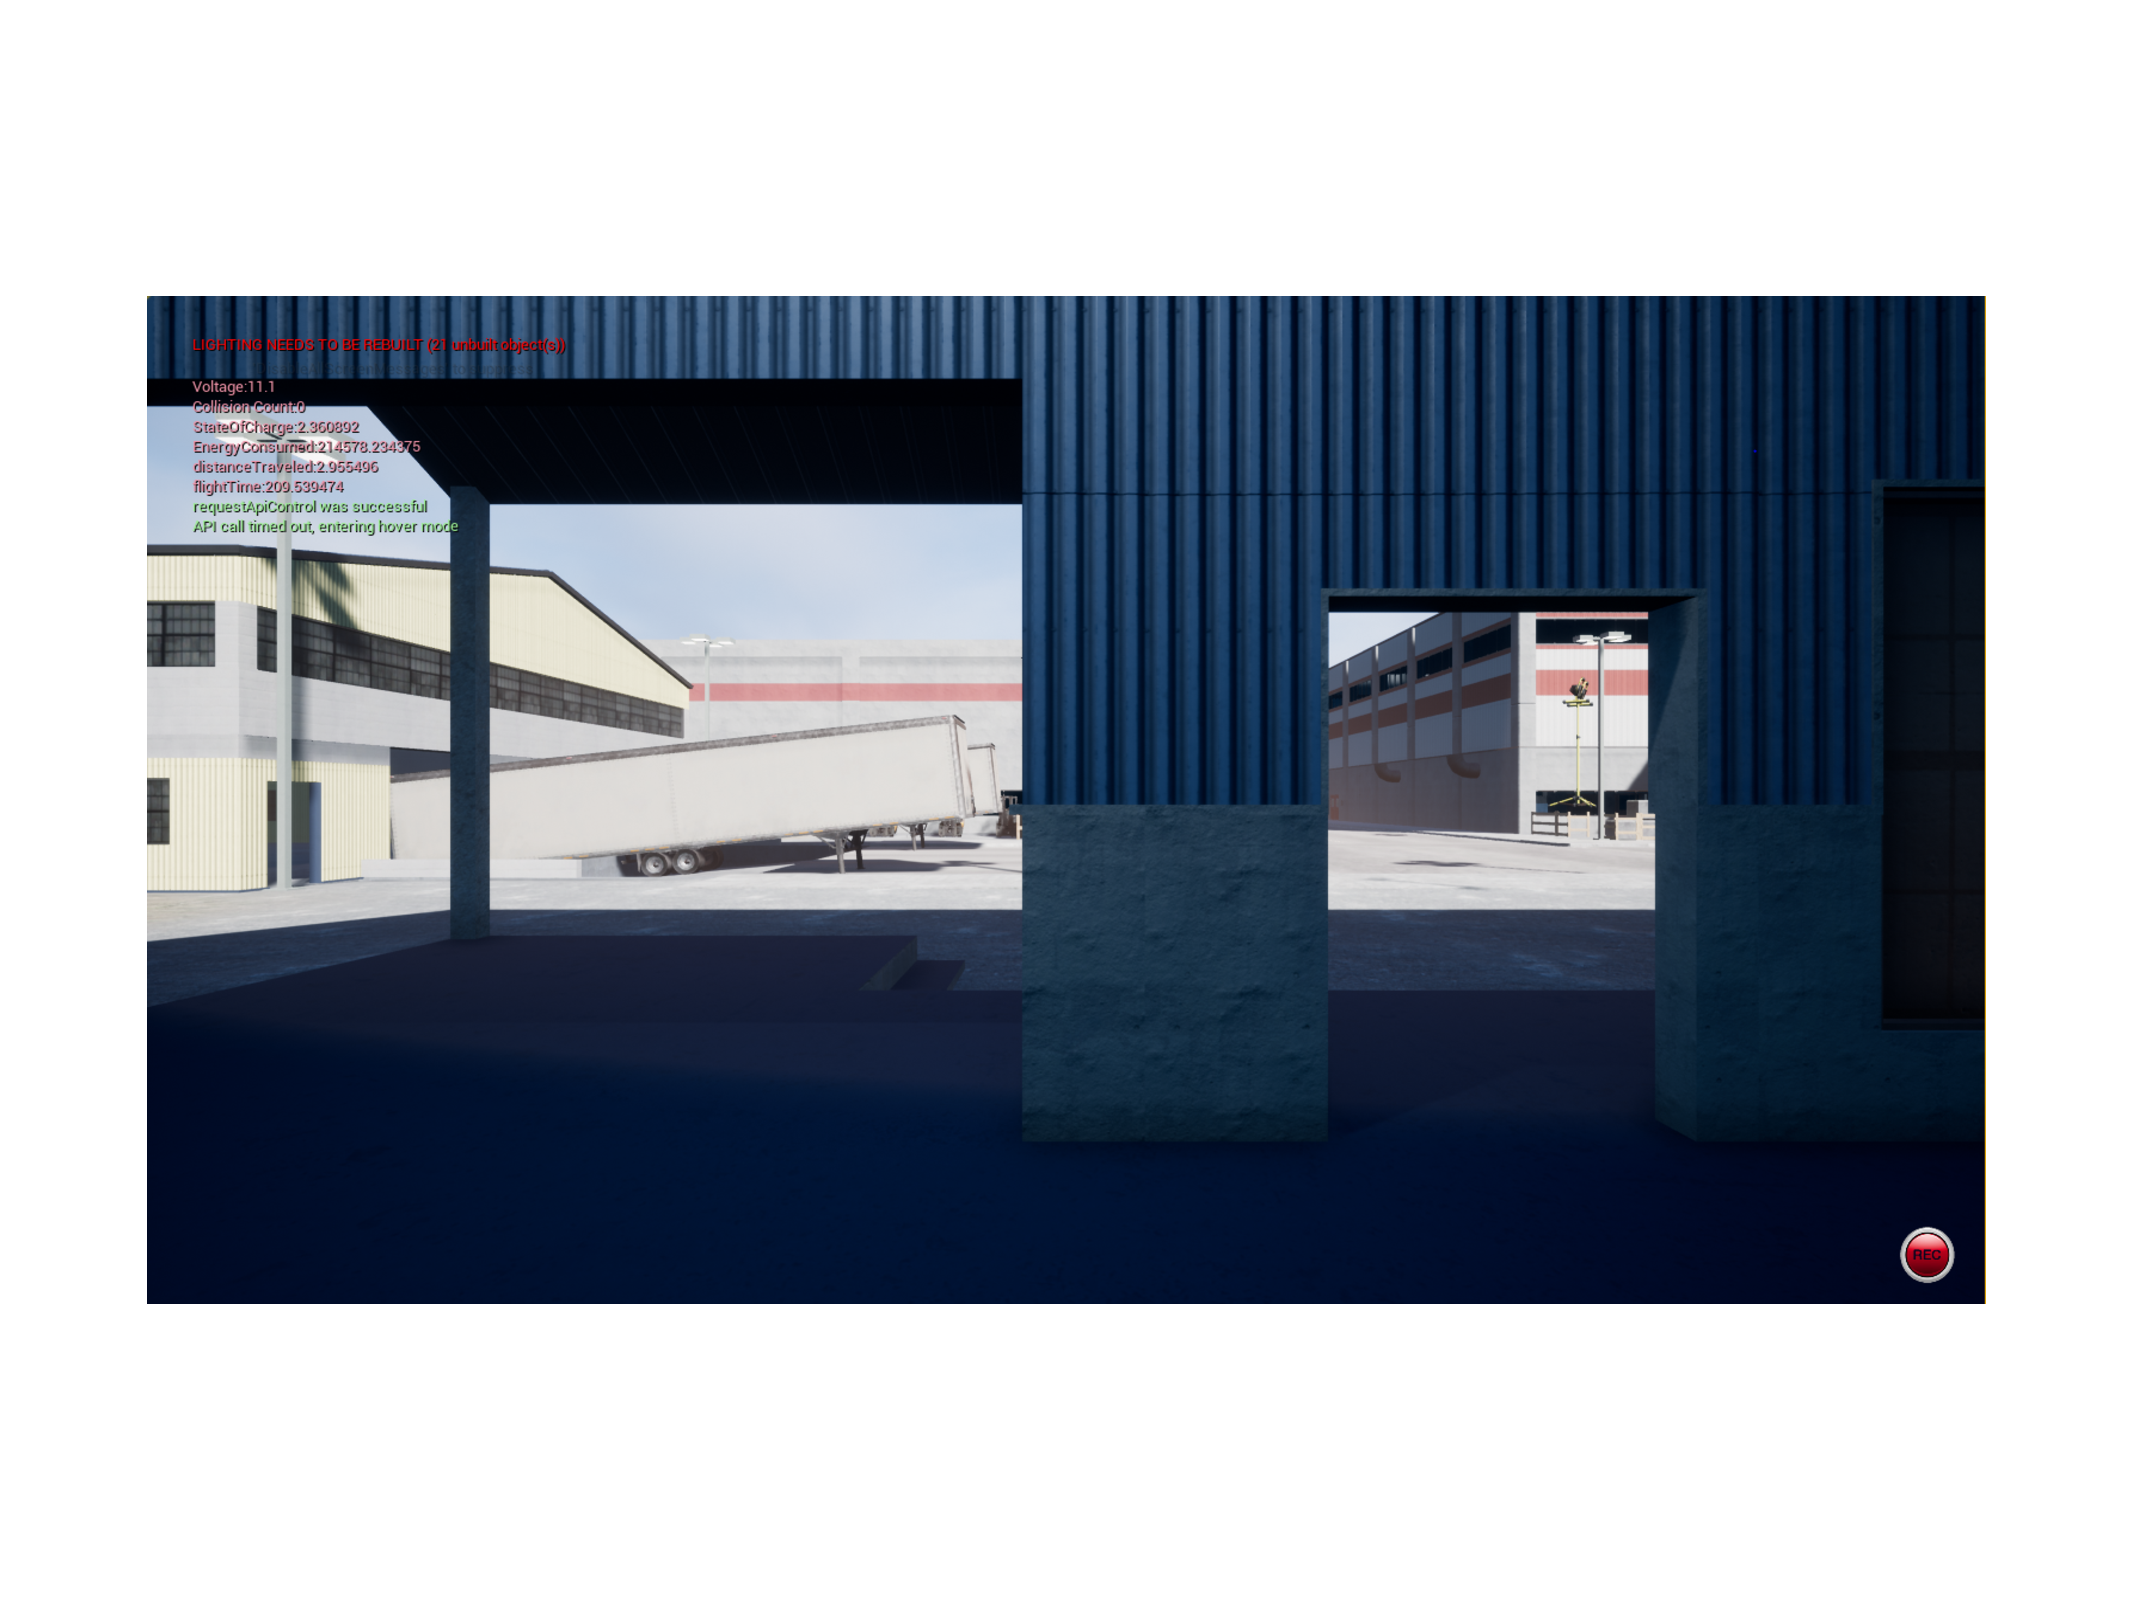
\includegraphics[trim=0 -10 0 -10, clip, width=\textwidth]{figs/garage_sim}
%DIFDELCMD <        \vspace{-30pt}
%DIFDELCMD <         %%%
%DIFDELCMD < \caption{%
{%DIFAUXCMD
\DIFdelFL{Environment's Map}}%DIFAUXCMD
%DIF < Level-1 Evaluation}
         %DIFDELCMD < 

%DIFDELCMD <         %DIFDELCMD < \label{fig:game:level-1}%%%
%DIFDELCMD <     \end{subfigure}
%DIFDELCMD <     \hfill
%DIFDELCMD <     \begin{subfigure}{.23\linewidth}
%DIFDELCMD <         \centering
%DIFDELCMD <         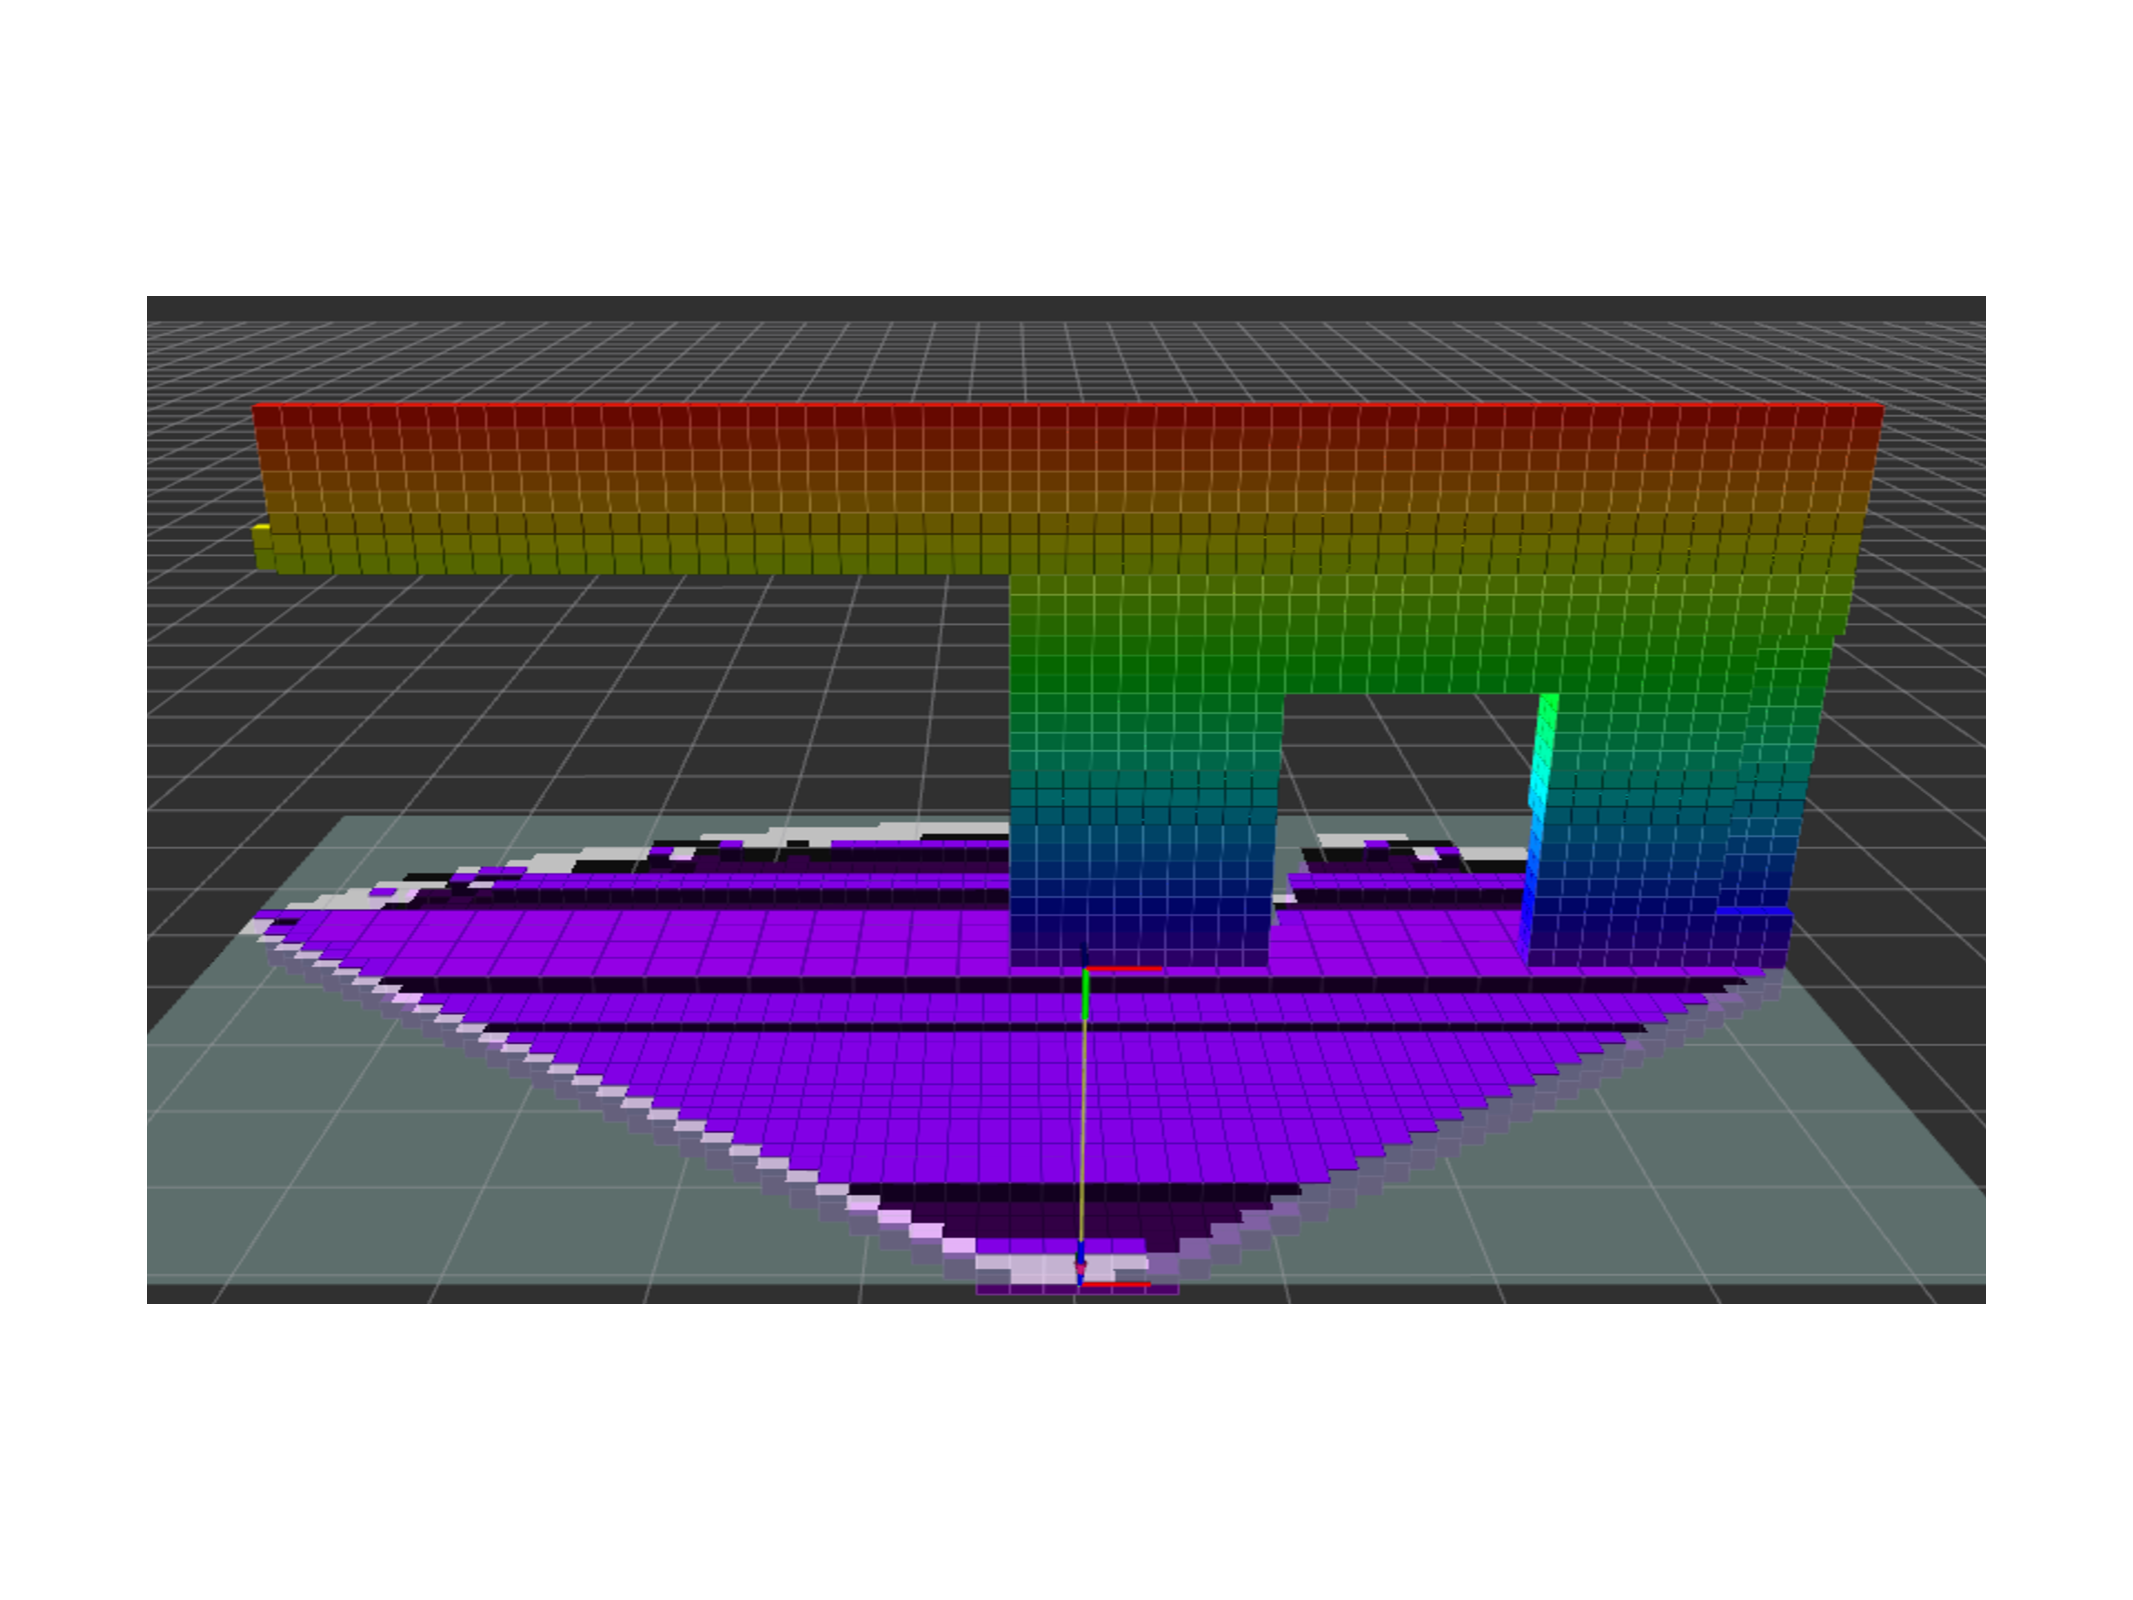
\includegraphics[trim=0 -10 0 -10, clip, width=\textwidth]{figs/garage_rviz__15}
%DIFDELCMD <        \vspace{-30pt}
%DIFDELCMD <        %%%
%DIFDELCMD < \caption{%
{%DIFAUXCMD
\DIFdelFL{resolution of .15 }\emph{\DIFdelFL{(m)}}%DIFAUXCMD
}
        %DIFAUXCMD
%DIFDELCMD < \label{fig:rviz__15}
%DIFDELCMD <     \end{subfigure}
%DIFDELCMD <     \hfill
%DIFDELCMD <      \begin{subfigure}{.23\linewidth}
%DIFDELCMD <         \centering
%DIFDELCMD <         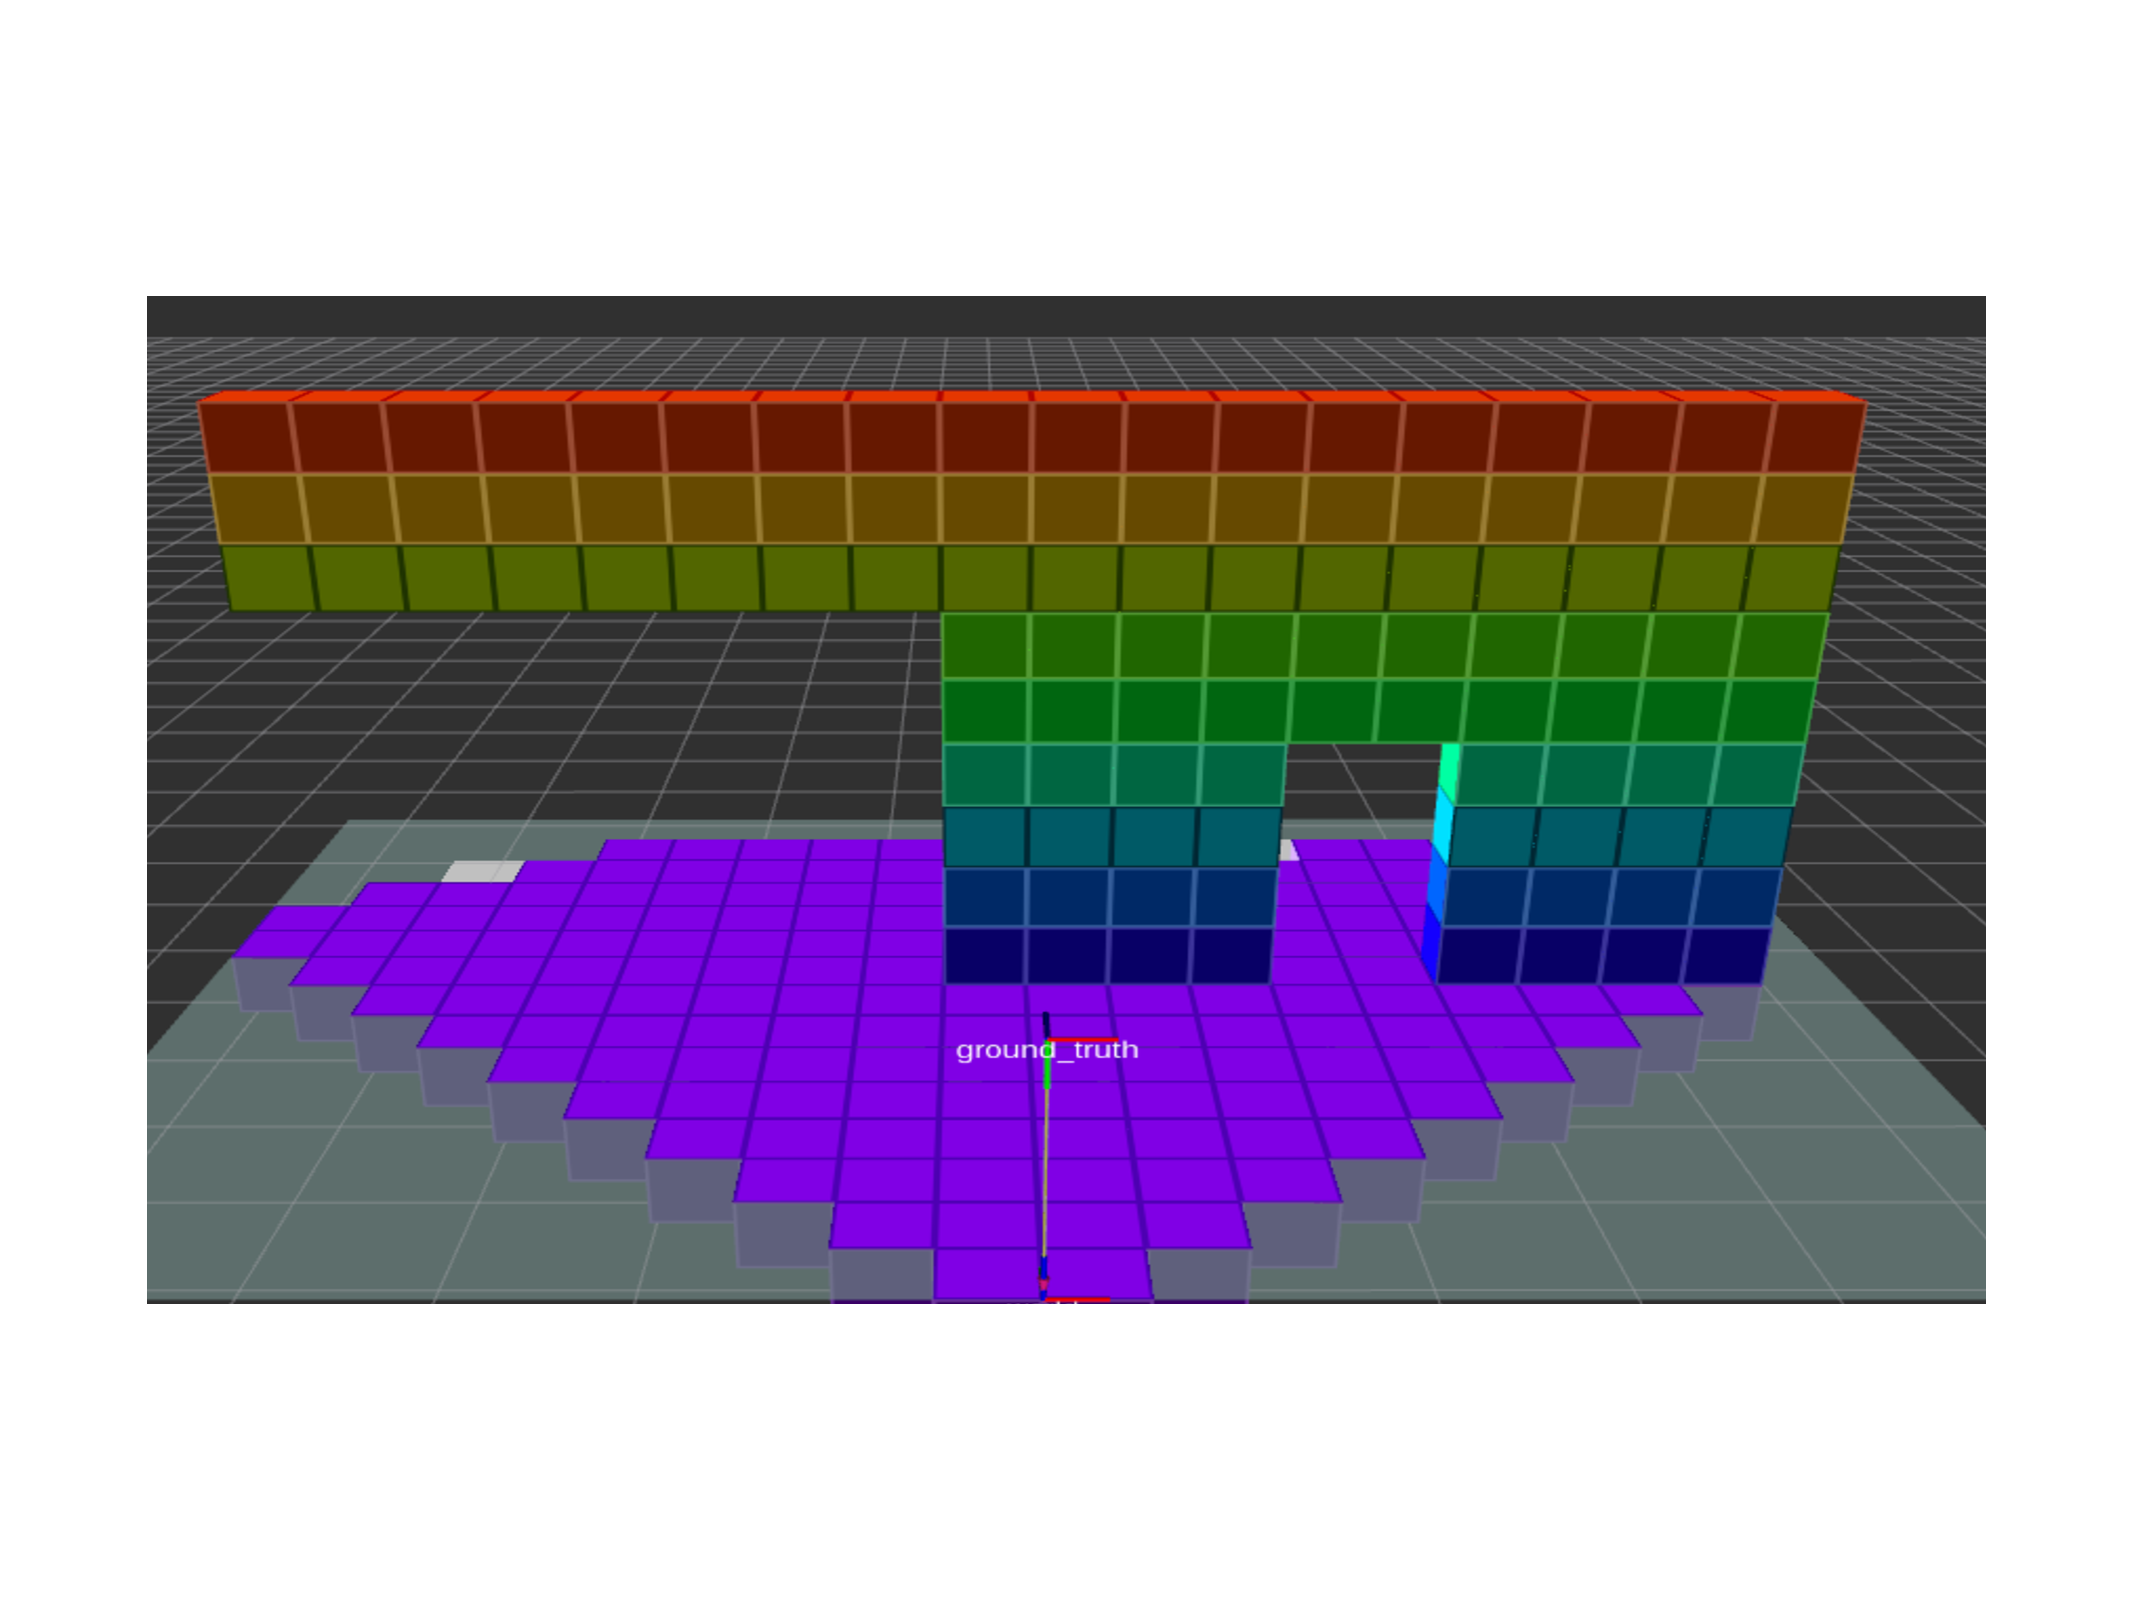
\includegraphics[trim=0 -10 0 -10, clip, width=\textwidth]{figs/garage_rviz__5}
%DIFDELCMD <        \vspace{-30pt}
%DIFDELCMD <        %%%
%DIFDELCMD < \caption{%
{%DIFAUXCMD
\DIFdelFL{resolution of .5 }\emph{\DIFdelFL{(m)}}%DIFAUXCMD
}
        %DIFAUXCMD
%DIFDELCMD < \label{fig:game:rviz__5}
%DIFDELCMD <     \end{subfigure}
%DIFDELCMD <        \hfill
%DIFDELCMD <    \begin{subfigure}{.23\linewidth}
%DIFDELCMD <         \centering
%DIFDELCMD <         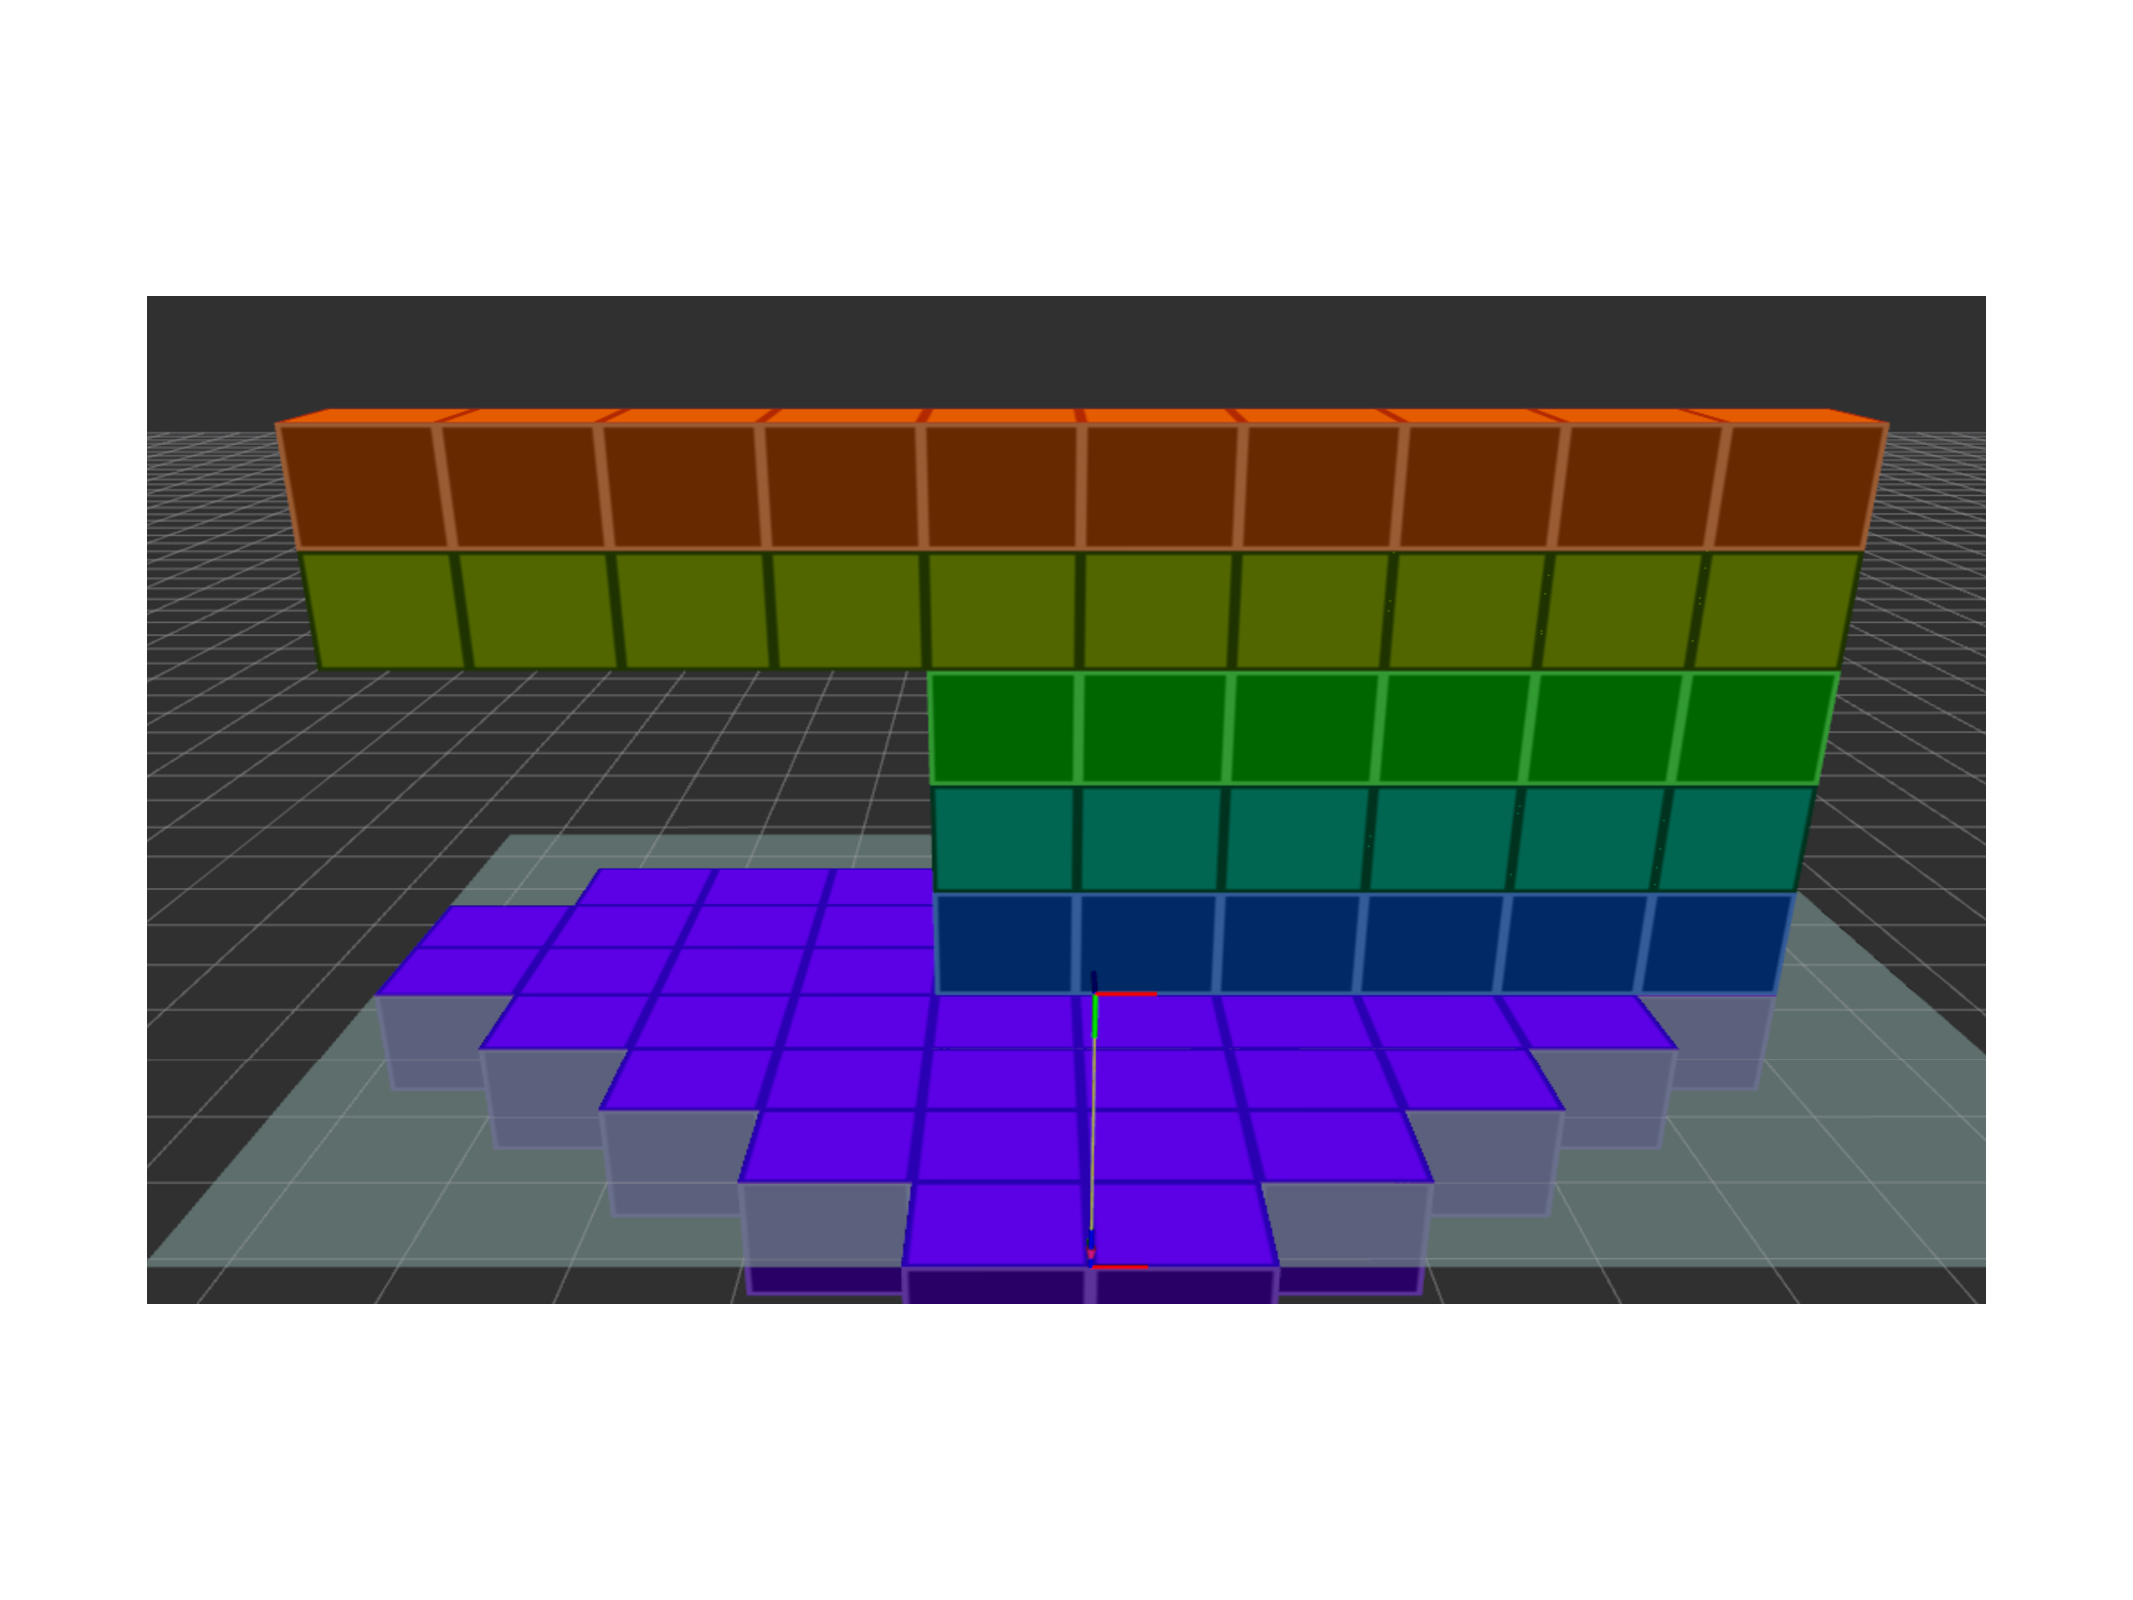
\includegraphics[trim=0 -10 0 -10, clip, width=\textwidth]{figs/garage_rviz_1}
%DIFDELCMD <         \vspace{-30pt}
%DIFDELCMD <         %%%
%DIFDELCMD < \caption{%
{%DIFAUXCMD
\DIFdelFL{resolution of .8 }\emph{\DIFdelFL{(m)}}%DIFAUXCMD
}%DIFAUXCMD
%DIF < Level-3 Evaluation}
        %DIFDELCMD < \label{fig:game:rviz_1}
%DIFDELCMD <     \end{subfigure}
%DIFDELCMD <     \hfill
%DIFDELCMD <    \vspace{+30pt}
%DIFDELCMD <    %%%
%DIFDELCMD < \caption{%
{%DIFAUXCMD
%DIFDELCMD < \small %%%
\DIFdelFL{Drone's environement }\emph{\DIFdelFL{(a)}} %DIFAUXCMD
\DIFdelFL{and its perception of it with various OctoMap resolutions (}\emph{\DIFdelFL{(b)}}%DIFAUXCMD
\DIFdelFL{, }\emph{\DIFdelFL{c}}%DIFAUXCMD
\DIFdelFL{, emph}%DIFDELCMD < {%%%
\DIFdelFL{d}%DIFDELCMD < }%%%
\DIFdelFL{).}}
    %DIFAUXCMD
%DIFDELCMD < \label{fig:octomap_perception}
%DIFDELCMD < \end{figure*}
%DIFDELCMD < 

%DIFDELCMD < %%%
\DIFdelend % Please add the following required packages to your document preamble:
% \usepackage{multirow}
\begin{table}[]
\vspace*{7pt}
\centering
\caption{Switching between OctoMap resolutions dynamically leads to mission success compared to 0.8~cm, and compared to 0.15~cm we consume less energy and thus retain more battery.}
\label{tbl:octopt}
\resizebox{1.0\columnwidth}{!}{
\begin{tabular}{l|l|l|l|}
\cline{2-4}
                                                                 & \textbf{Resolution {(cm)}}       & \textbf{Mission Status} & \textbf{Battery  (\%)} \\ \hline
\multicolumn{1}{|l|}{\multirow{3}{*}{\textbf{Package Delivery}}} & \textit{0.8}              & \cellcolor{red!25}Fail                    &   0           \\ \cline{2-4} 
\multicolumn{1}{|l|}{}                                           & \textit{0.15}             & Pass                    &    81.00          \\ \cline{2-4} 
\multicolumn{1}{|l|}{}                                           & \textit{Chameleon (0.8, 0.15)} & Pass                    &   \cellcolor{green!25}86.00           \\ \hline
\multicolumn{1}{|l|}{\multirow{3}{*}{\textbf{Mapping}}}          & \textit{0.8}              & \cellcolor{red!25}Fail                    & 0           \\ \cline{2-4} 
\multicolumn{1}{|l|}{}                                           & \textit{0.15}             & Pass                    & 39.03        \\ \cline{2-4} 
\multicolumn{1}{|l|}{}                                           & \textit{Chameleon (0.8, 0.15)} & Pass                    & \cellcolor{green!25}53.83        \\ \hline
\multicolumn{1}{|l|}{\multirow{3}{*}{\textbf{Search and Rescue}}}              & \textit{0.8}              & \cellcolor{red!25}Fail                    & 0         \\ \cline{2-4} 
\multicolumn{1}{|l|}{}                                           & \textit{0.15}             & Pass                    & 24.21        \\ \cline{2-4} 
\multicolumn{1}{|l|}{}                                           & \textit{Chameleon (0.8, 0.15)} & Pass                    & \cellcolor{green!25}57.87        \\ \hline
\end{tabular}
}
\end{table}

Size of the voxels, i.e. the map's resolution, trades off accuracy and flight-time/energy. By lowering the resolution, i.e. increasing voxel sizes, obstacle boundaries get inflated, hence the drones perception of the environment and the objects within it becomes inaccurate. However, doing so improves the performance of the OctoMap node and eventually leads to a faster flight time. To examine the trade off, we ran OctoMap with various resolutions.
\DIFdelbegin %DIFDELCMD < \Fig{fig:octrest} %%%
\DIFdel{shows 4.5X speed up in the OctoMap's update rate for 6.5X reduction in accuracy. 
%DIF < \begin{comment}
}%DIFDELCMD < 

%DIFDELCMD < %%%
%DIF < \end{comment}
\DIFdelend %DIF > \Fig{fig:octrest} shows 4.5X speed up in the OctoMap's update rate for 6.5X reduction in accuracy. 
\DIFaddbegin \begin{comment}
\begin{figure}[b]
\centering
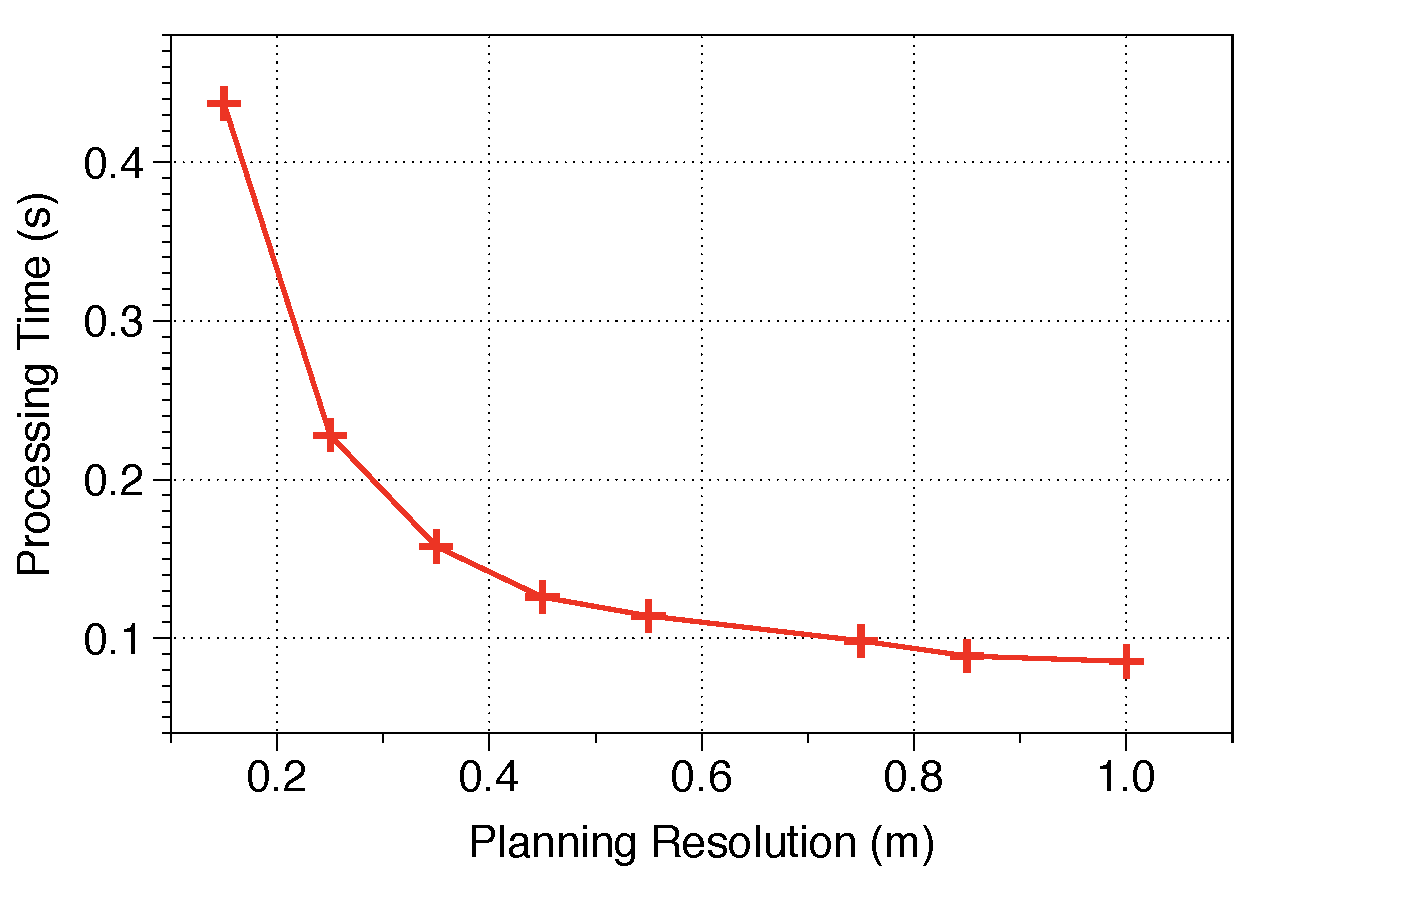
\includegraphics[trim=0 0 0 -25, clip, width=\columnwidth]{figs/octomap_resolution_case_study}
\caption{OctoMap accuracy (resolution) versus performance.}
\label{fig:octrest}
\end{figure}
\end{comment}
\DIFaddend Certain aspects of the environment such as obstacle density determine the OctoMap resolution. In low density environments, where the drone has ample opportunities for paths to take, a low resolution can suffice. However, in dense environments, low resolutions can deprive the drone from path opportunities present since the drone perceive the obstacles bigger than they are. \DIFdelbegin %DIFDELCMD < \red{The impact of OctoMap resolution on the drone's perception can be easily seen in figure blah, where figure blah-1 shows the environment and the figure blah-2 through 4 show the drone's perception of the environment. As observed, when the resolution is lowered, the voxel sizes increase to the point that the drone can fail to recognize openings as possible passage ways to plan through. This in turn can result in a mission inefficiency and possible failures depending on the environment}%%%
\DIFdel{.
}\DIFdelend Since the environment around the drone changes, a dynamic approach where the resolution is set on the runtime is desirable. We study two environments during the mission, namely outdoors (low obstacle density) and indoors (high obstacle density). 

Table~\ref{tbl:octopt} shows the result of two static (predetermined) resolutions, 15~cm and 80~cm, and our proposed dynamic approach (Chameleon) that multiplexes between the two appropriately. The dynamic approach allows for up to 2.3X improvement in endurance. As compute reduces, OctoMap bottleneck eases, and therefore the drone completes its mission faster. 

The table also highlights another interesting relationship. Statically choosing the 80~cm resolution to optimize for compute (only) causes the drone to fail its mission since it is unable to plan paths through narrow openings in the indoor environments. By switching between two resolutions according to the environments obstacle density, Chameleon is able to balance OctoMap computation with mission feasibility and energy, holistically. Therefore, in all cases, Chameleon uses less energy and retains more battery charge. \DIFdelbegin %DIFDELCMD < 

%DIFDELCMD < \red{\subsection{Depth Sensor Noise: A Reliability Case-Study}}
%DIFDELCMD < \red{Vijay could you add the information flow introduction you mentioned.}
%DIFDELCMD < 

%DIFDELCMD < \red{In this case study we examined the impact of sensor noise on the performance of our package delivery application. We injected Gaussian noise with a range of standard deviations into the depth readings of the drone's RGBD camera. Sensory noise distorts the drone's perception of the obstacles in its environment, and we found that Gaussian noise in particular \emph{inflates} obstacles, making them appear larger than they actually are. This causes the drone to re-plan its trajectories more often, as it assumes that its planned path will collide into objects that are actually further away than they seem, as shown in figure blah. The more the drone re-plans its paths, the longer it takes to reach its destination, increasing mission time by blah percent.
%DIFDELCMD < }
%DIFDELCMD <  %%%
\DIFdelend